\documentclass{beamer}				% Präsentation
\usetheme{Warsaw}
%\usetheme{Copenhagen}					% Layout, siehe https://hartwork.org/beamer-theme-matrix/
\usecolortheme{orchid}				% Farbdesign, siehe https://hartwork.org/beamer-theme-matrix/
\usepackage[utf8]{inputenc}			% UTF8 Encoding
\usepackage[german=quotes]{csquotes}% Deutsche Anführungszeichen über \enquote{}
\usepackage{amsmath}				% Mathe Support
\usepackage{amsfonts}				% Mathe Schriftarten
\usepackage{amssymb}				% Mathe Symbole
\usepackage{pgfplots}				% Graphen
\pgfplotsset{compat=1.14} 			% Graph Kombatibilität mit den Uni PCs
\usepackage{tabularx}				% Tabellen
\usepackage{pgfpages}
\usepackage{hyperref}
\usepackage[export]{adjustbox} 

\defbeamertemplate{footline}{author and frame number}{%
	\usebeamercolor[fg]{frame number in head/foot}%
	\usebeamerfont{frame number in head/foot}%
	\hspace{1em}\insertshortauthor\hfill%
	\insertframenumber\,/\,\inserttotalframenumber\kern1em\vskip2pt%
}

\setbeamertemplate{footline}[author and frame number]
\beamertemplatenavigationsymbolsempty
\graphicspath{ {images/} }
\author{Marcel Richter und Vanessa Speeth}
\date{28.05.2019}
\title{Unity Projekt 2: Zwischenstand}


\begin{document}
	\begin{frame}[noframenumbering,plain]
	\titlepage
	\end{frame}


	\begin{frame} {Themengebiet}
			\begin{itemize}
				\item Inventar
				\item User Interface
				\item Crafting System
			\end{itemize}
	\end{frame}

	\begin{frame}{Bisherige Erfolge UI}
		\begin{itemize}
			\item HotKeys unterhalb des Bildschirms
			\item Inventar Design
			\item ToolTip für die Itembeschreibung bei Hover
			\item Drag \& Drop innerhalb des Inventars
			\item HotKeys aktualisieren sich sobald sie im Inventar-Fenster befüllt werden
			\item Drag \& Drop außerhalb des Inventars führt zum entfernen des Items
	\end{itemize}
	\end{frame}

	\begin{frame}{Weitere Erfolge}
	\begin{itemize}
		\item Verkleinern von Chunks nach dem Abbauen	
		\item Items als Scriptable Objects
		\item Rezepte als Scriptable Objects
	\end{itemize}
\end{frame}
	\begin{frame}{HotKeys}
	\centering
	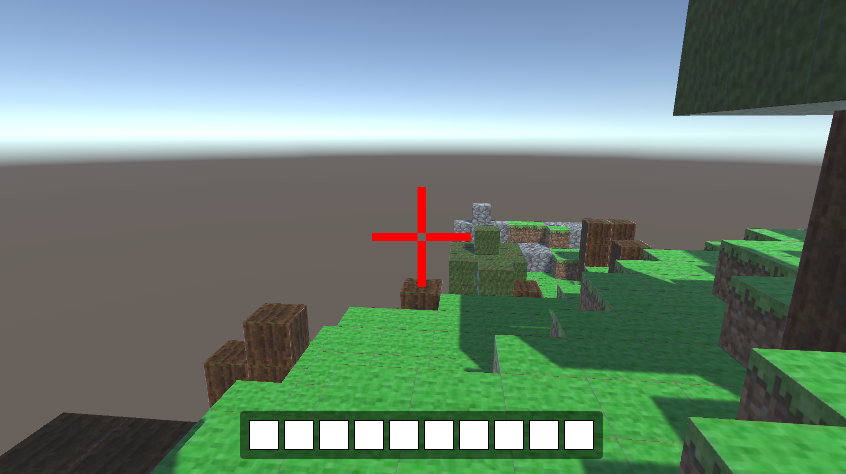
\includegraphics[height=6cm]{Hotkeys}
	\end{frame}
	
	\begin{frame}{Inventar}
	\centering
	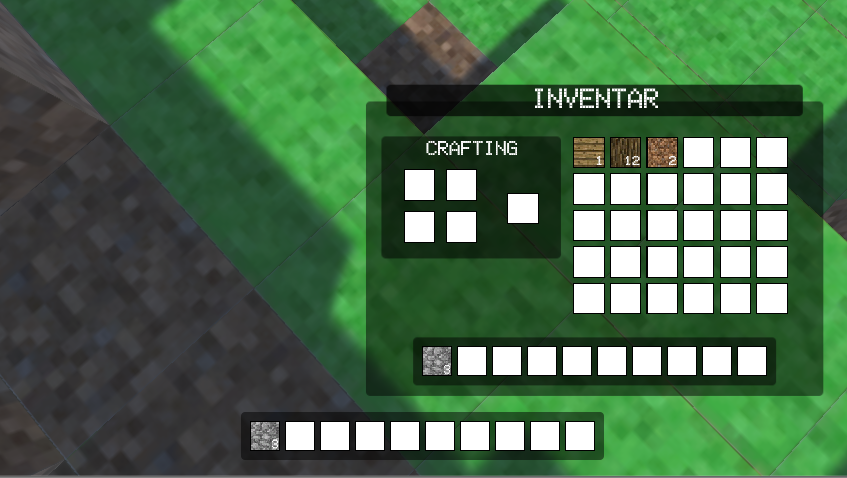
\includegraphics[height=6cm]{InventoryOpen}
	\end{frame}
	
	\begin{frame}{Verbotene Drops}
	\centering
	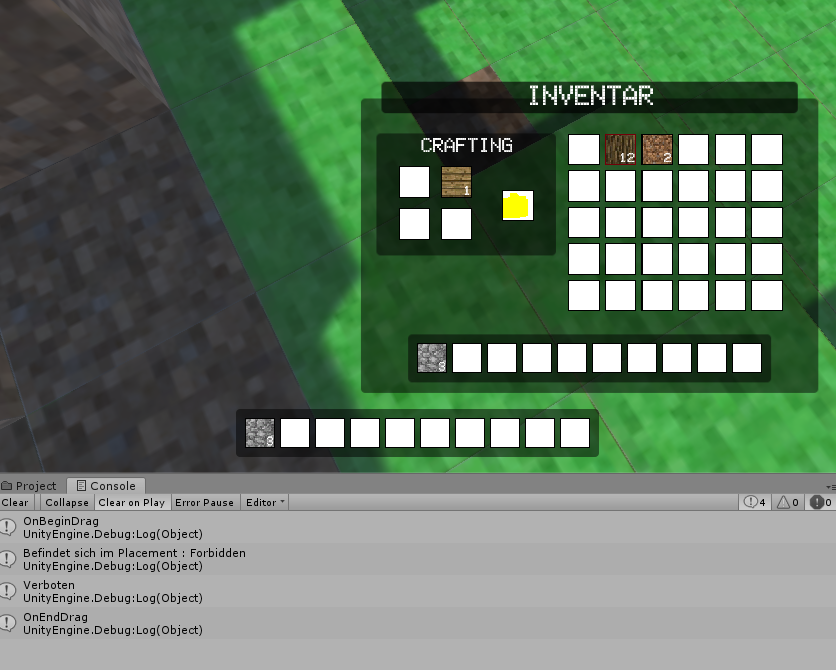
\includegraphics[height=6cm]{Forbidden}
	\end{frame}
	
	\begin{frame}{Werwerfen von Items}
	\centering
	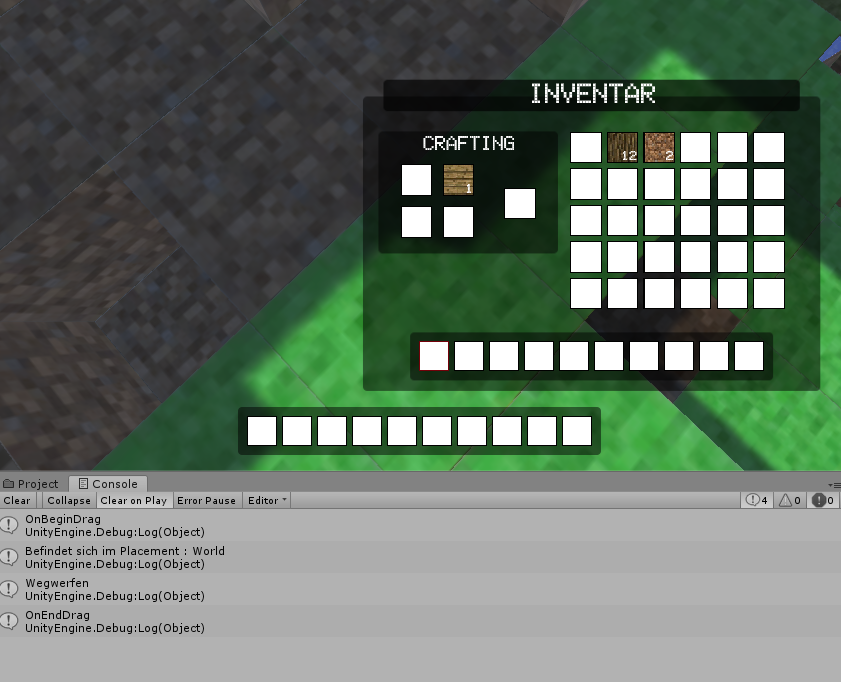
\includegraphics[height=6cm]{ThrowAway}
	\end{frame}
	
	\begin{frame}{Verkleinern von Chunks nach dem Abbauen}
	\centering
	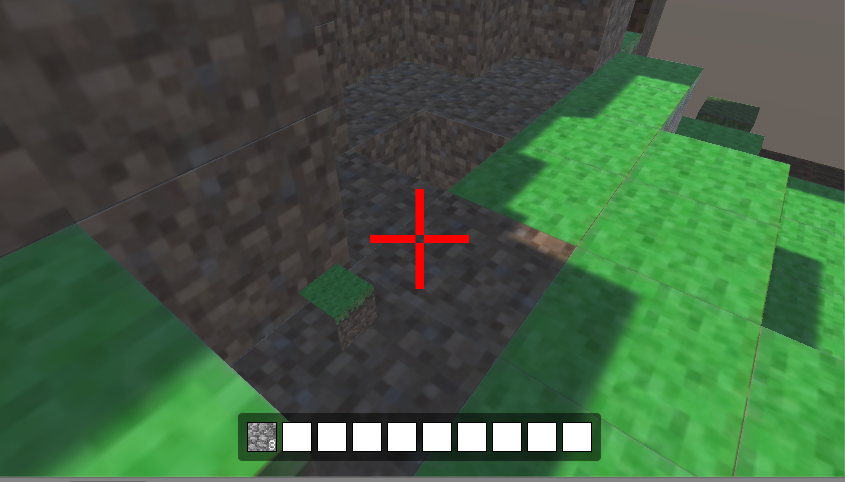
\includegraphics[height=6cm]{SmallChunk}
	\end{frame}
	
	\begin{frame}{Weitere Ziele}
		\begin{itemize}
			\item Einsammeln von abgebauten Items
			\item Rezepte für Crafting als Rezeptbuch anzeigen
			\item Neue Items erstellen und speichern (gecraftete Items)
			\item HotKeys sollen auf Zahlenreihe reagieren 
			\item Bauen von Items aus dem Inventar
		\end{itemize}
	\end{frame}

\end{document}
